\documentclass[compress]{beamer}
\usepackage[utf8]{inputenc}
\usepackage[english]{babel}
\usepackage{hyperref}
\usepackage{ccicons}

\usepackage{tikz}
\usetikzlibrary{graphs, quotes, arrows.meta, matrix}

\newcommand\scalemath[2]{\scalebox{#1}{\mbox{\ensuremath{\displaystyle #2}}}}

\usetheme{default}
\usecolortheme{Nord}
\setbeamertemplate{navigation symbols}{}

\title{Teoria dei grafi}
\subtitle{Algoritmi classici}
\author{Lorenzo Ferrari, Davide Bartoli}
\date{\today}

\begin{document}

\begin{frame}
  \maketitle
\end{frame}

\begin{frame}{Table of contents}
  \tableofcontents
\end{frame}

\section{Dijkstra}
\subsection{Problema}
\begin{frame}{Dijkstra}{Problema}
    \begin{exampleblock}{Single source shortest path}
        Dato un grafo $G = (V, E)$ \textbf{pesato}, trovare la minima distanza tra due nodi $a$ e $b$, ovvero il percorso 
        di peso totale minimo che parte da $a$ e arriva a $b$.
    \end{exampleblock}
    \pause
    Supponiamo che il grafo non sia pesato.
    \begin{itemize}
        \item potremmo usare l'algoritmo di \textbf{BFS} per trovare il percorso pi\`u corto
        \item in queso caso la \textbf{BFS} funziona dato che visita i nodi in ordine di distanza crescente
    \end{itemize}
    \pause
    Riusciamo in qualche modo a visitare i nodi in ordine di distanza crescente anche con il grafo pesato?
\end{frame}

\begin{frame}{Dijkstra}{Problema}
    Vorremmo avere una struttura dati equivalente a una coda, ma che ordini i nodi in base alla distanza dal nodo sorgente.
    Per nostra fortuna questa ds esiste già all'interno della libreria standard di C++: \textbf{std::priority\_queue}.
    \pause
    \begin{exampleblock}{Dijkstra}
        \begin{itemize}
            \item inizializziamo la distanza del nodo sorgente a 0
            \pause
            \item aggiungiamo il nodo sorgente alla priority\_queue
            \pause
            \item finch\`e la priority\_queue non \textbf{\`e vuota}:
                \begin{itemize}
                    \item estraiamo il nodo con distanza minima dalla coda
                    \pause
                    \item per ogni nodo adiacente a quello estratto:
                        \begin{itemize}
                            \item se posso migliorare la sua distanza, la aggiorno e lo aggiungo alla priority\_queue
                        \end{itemize}
                \end{itemize}
        \end{itemize}
        \pause
        La complessit\`a di questo algoritmo \`e $O((N + M) \cdot log N)$, dato che la priority\_queue ha complessit\`a $O(log N)$ per ogni operazione.
    \end{exampleblock}
\end{frame}

\subsection{Implementazione}
\begin{frame}{Dijkstra}{Implementazione}
    \makebox[\textwidth]{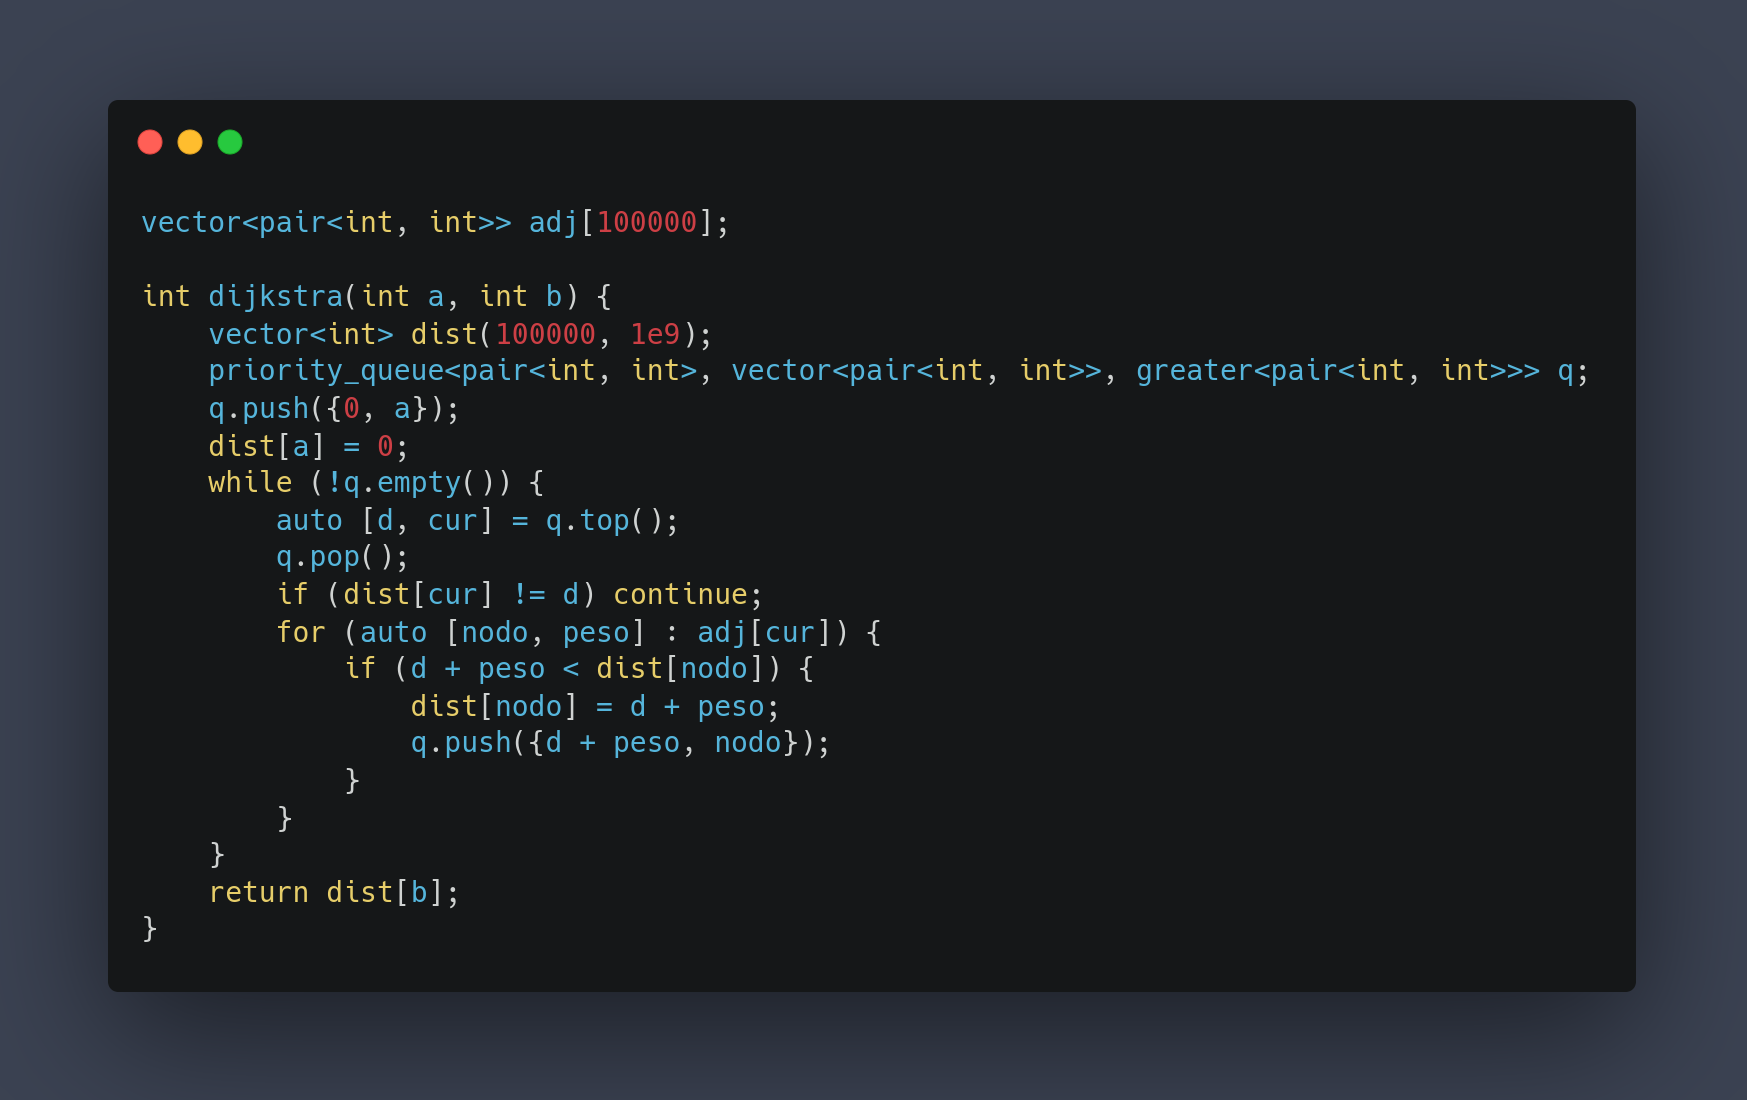
\includegraphics[scale=.2]{./img/dijkstra1.png}}
\end{frame}

\begin{frame}{Dijkstra}{Implementazione}
    \makebox[\textwidth]{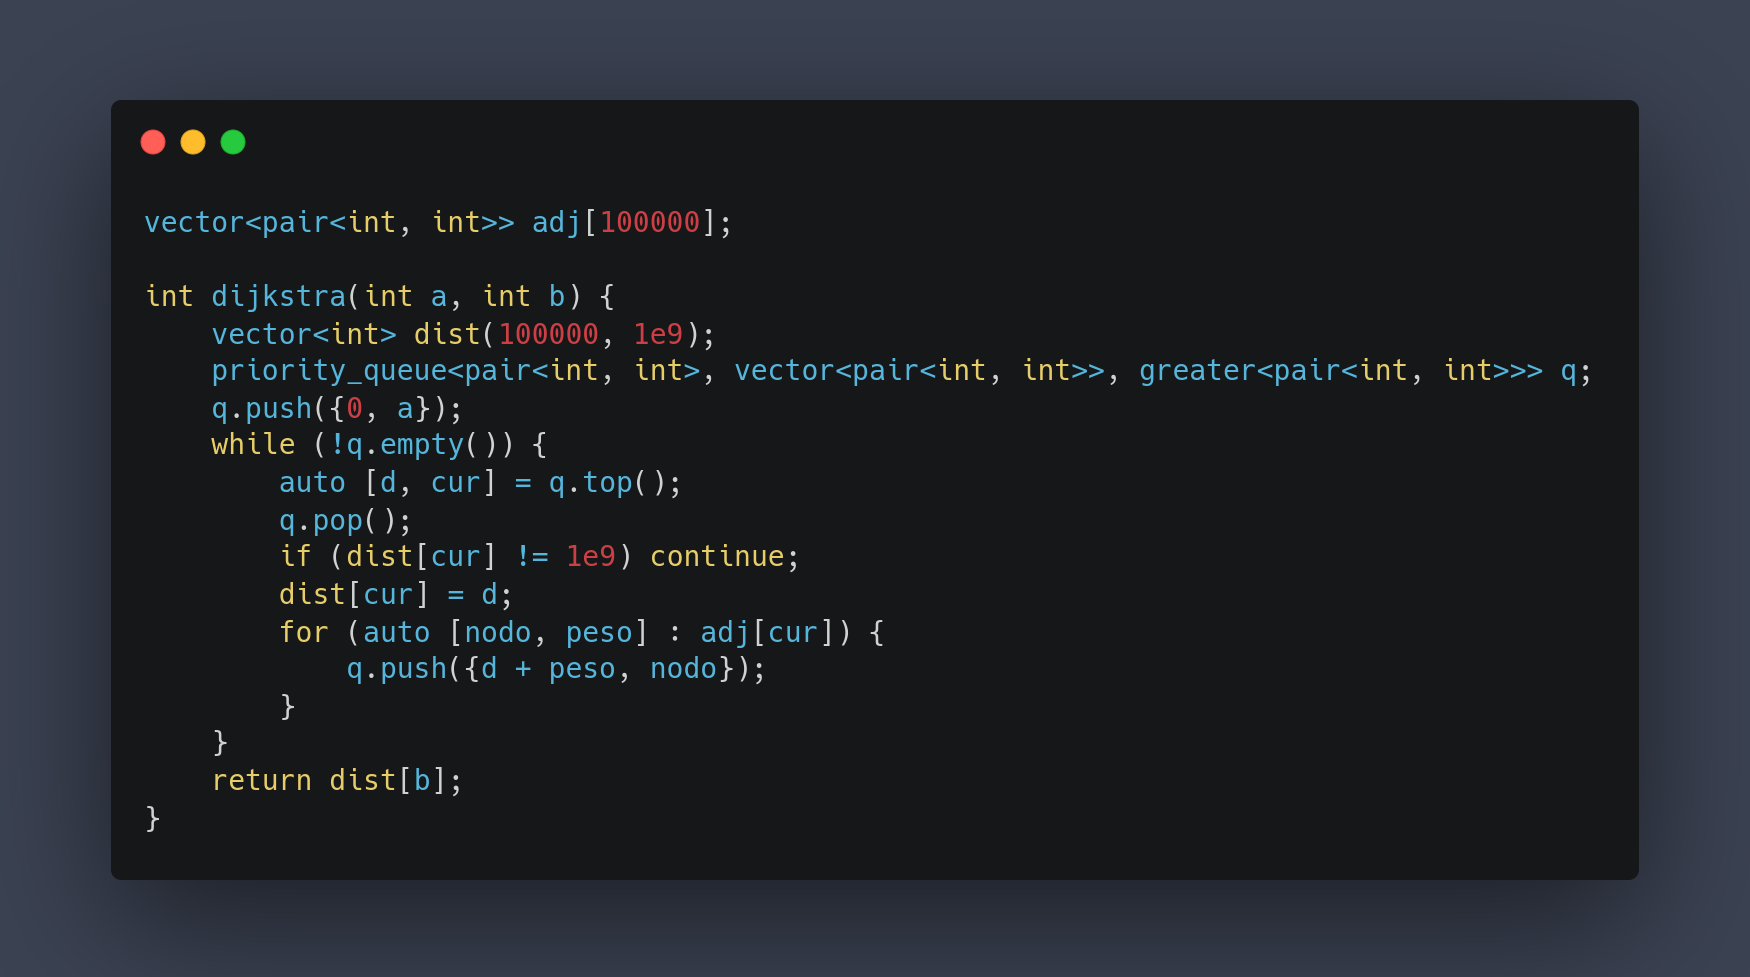
\includegraphics[scale=.2]{./img/dijkstra.png}}
\end{frame}


\begin{frame}{Dijkstra}{Osservazione}
    Dijkstra non funziona se sono presenti archi con peso negativo.
    \pause 
    \begin{itemize}
        \item se è presente un ciclo negativo, l'algoritmo può andare in loop infinito
        \pause
        \item anche se non è presente un ciclo negativo, l'algoritmo può non trovare il percorso minimo o 
        avere una complessità fino a esponenziale a seconda delle implementazioni
    \end{itemize}
    \pause
    Se il grafo è denso ($M = O(N^2)$), possiamo implementare Dijkstra in modo naive e otterene una complessit\`a leggermente migliore.
\end{frame}

\section{Disjoint Set Union}
\subsection{Problema}
\begin{frame}{Disjoint Set Union}{Problema}
    \begin{exampleblock}{Contare le componenti connesse online}
        Dati $n \leq 10^6$ nodi e $m \leq 10^6$ update che aggiungono un arco $(a_i, b_i)$, dire dopo ogni update quante componenti connesse ci sono.
    \end{exampleblock}
    \pause
    \begin{itemize}
        \item un'opzione \`e fare $M$ visite ognuna in $O(N + M)$, ma quest'approccio prenderebbe sicuramente TLE (Time Limit Exceeded)
        \pause
        \item al momento non sappiamo risolverlo efficientemente
        \pause
        \item servirebbe una struttura dati che rappresenti ogni componente connessa e che sia in grado di unire due componenti connesse efficientemente
    \end{itemize}
\end{frame}

\begin{frame}{Disjoint Set Union}{Idea}
    La struttura dati \textbf{Disjoint Set Union} (spesso chiamata anche \textbf{Union Find}) fa esattamente questo.
    In particolare, implementeremo le seguenti operazioni:
    \pause
    \begin{itemize}
        \item \texttt{find(v)}, trova un nodo nella componente connessa di \texttt{v}
            \pause
            \begin{itemize}
                \item vogliamo che \texttt{find(v)} ritorni lo stesso nodo per tutti i \texttt{v} appartenenti alla stessa componente connessa
                \item per il \textit{rappresentante} di una componente connessa vale \texttt{find(v)~==~v}
            \end{itemize}
        \pause
        \item \texttt{merge(a, b)}, aggiungi l'arco \texttt{(a, b)}
    \end{itemize}
    \pause
    \begin{alertblock}{}
        La connettivit\`a non cambia se, invece dell'arco \texttt{(a, b)}, si aggiunge l'arco \texttt{(find(a), find(b))}
    \end{alertblock}
\end{frame}

\subsection{Implementazione}
\begin{frame}{Disjoint Set Union}{Implementazione}
    \begin{itemize}
        \item manteniamo una foresta, in cui ogni albero corrisponde a una componente connessa
        \item la radice dell'albero \`e il nodo rappresentante della componente
        \item inizialmente ci sono $n$ alberi ognuno composto da un unico nodo
        \item per ogni nodo \texttt{v}, salviamo il suo parent \texttt{par[v]}\footnote{per la radice vale \texttt{par[v] == v}}
    \end{itemize}
\end{frame}

\begin{frame}{Disjoint Set Union}{Struttura}
    \makebox[\textwidth]{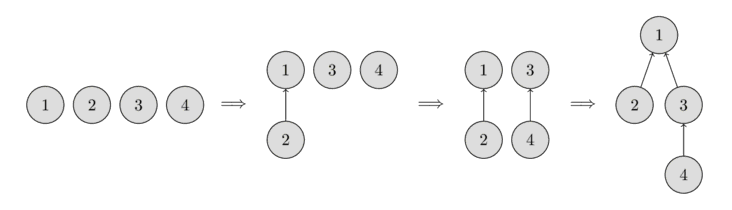
\includegraphics[scale=.45]{./img/dsu_example.png}}
\end{frame}

\begin{frame}[plain]
    \makebox[\textwidth]{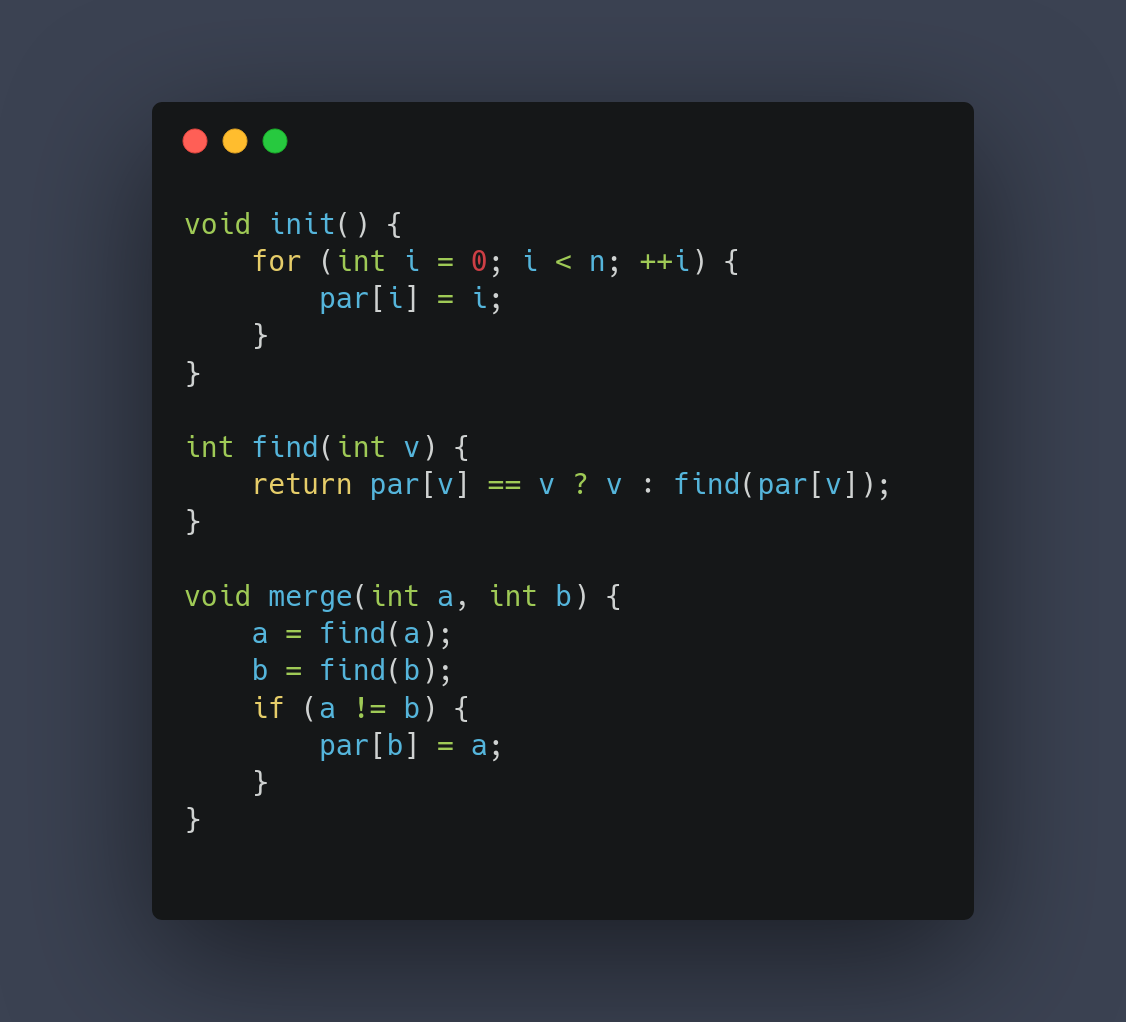
\includegraphics[scale=.25]{./img/dsu_naive.png}}
\end{frame}

\begin{frame}{Disjoint Set Union}{Complessit\`a}
    La struttura dati funziona, ma \`e abbastanza efficiente?
    \pause
    \begin{block}{Complessit\`a}
    \begin{itemize}
        \item la complessit\`a di tutte le operazioni dipende dall'altezza $h$ dell'albero
    \end{itemize}
    \end{block}
    \pause
    Si pu\`o dimostrare che, se gli archi sono inseriti in ordine casuale, l'altezza massima attesa \`e $O(\log n)$.
    Tuttavia esiste il caso pessimo in cui l'albero \`e una catena: in quel caso ogni operazione costa $O(h) = O(n)$.
    \pause

    Si pu\`o fare meglio di cos\`i?
\end{frame}

\subsection{Ottimizzazioni}
\begin{frame}{Disjoint Set Union}{Path compression}
    \begin{block}{Idea}
        se in qualunque momento cambiamo \texttt{par[v]} in \texttt{par[v] = find(v)}, la connettivit\`a non cambia, ma le prossime chiamate a \texttt{find(v)} saranno pi\`u veloci.
    \end{block}
    Ad ogni chiamata di \texttt{find(v)}, aggiorniamo il parent anche di tutti i suoi antenati.
    \vfill
    Con quest'ottimizzazione la complessit\`a ammortizzata\footnote{complessit\`a ammortizzata $O(f(x))$ significa che la somma di $m$ operazioni \`e $O(m f(x))$} diventa $O(\log n)$
\end{frame}

\begin{frame}{Disjoint Set Union}{Path compression}
    \makebox[\textwidth]{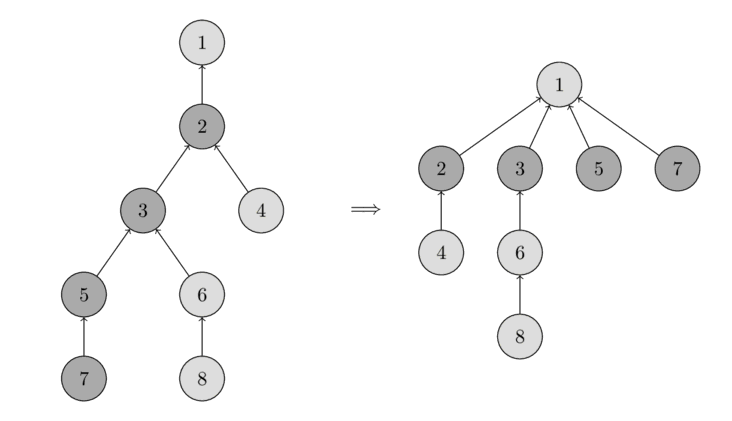
\includegraphics[scale=.4]{./img/dsu_path_compression.png}}
\end{frame}

\begin{frame}{Disjoint Set Union}{Implementazione}
    \makebox[\textwidth]{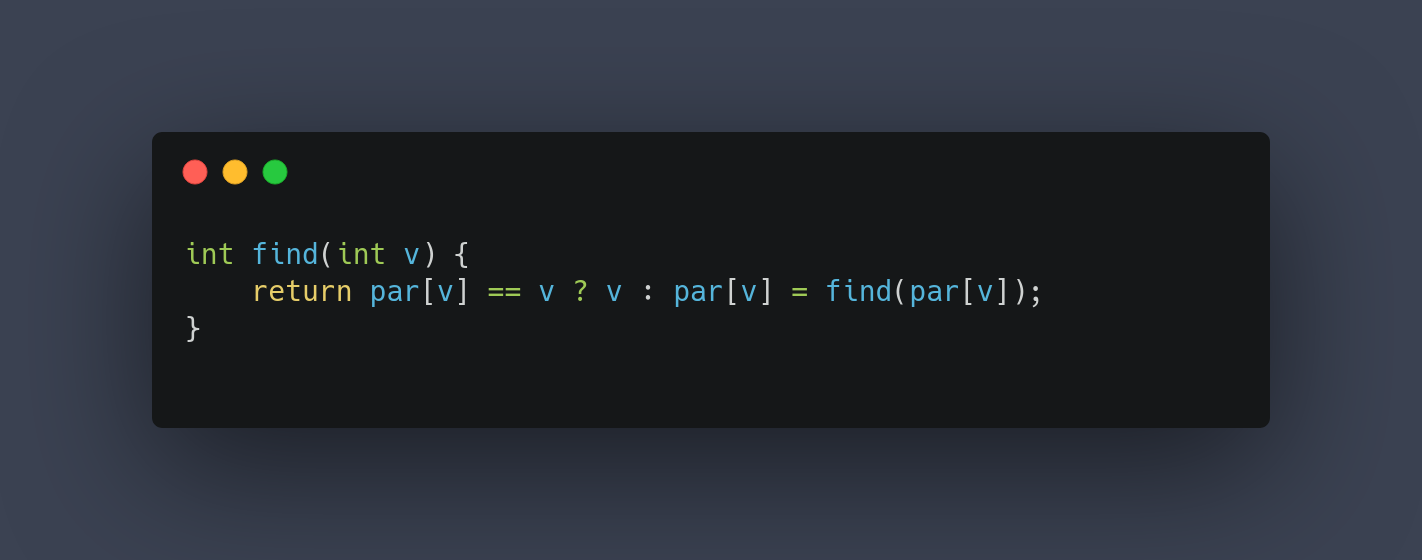
\includegraphics[scale=.3]{./img/path_compression.png}}
\end{frame}

\begin{frame}{Disjoint Set Union}{Ottimizzazioni}
    Se uniamo sempre l'albero pi\`u ``piccolo'' in quello pi\`u ``grande'', si dimostra che l'altezza massima di un albero con $n$ nodi \`e al pi\`u $\log n$.
    \begin{block}{Union by rank}
        \begin{itemize}
            \item salviamo in ogni radice l'altezza \texttt{rank[v]} dell'albero
            \item il rank aumenta solo quando mergiamo due alberi dello stesso rank
            \item per induzione si dimostra che un albero con $\texttt{rank[v]} = h$, ha almeno $2^h$ nodi
            \item $h = O(\log n)$
        \end{itemize}
    \end{block}
\end{frame}

\begin{frame}{Disjoint Set Union}{Ottimizzazioni}
    \begin{block}{Union by size}
        \begin{itemize}
            \item salviamo in ogni radice il numero di nodi \texttt{size[v]} nel suo albero
            \item dopo ogni operazione \texttt{merge}, il nuovo albero ha almeno il doppio dei nodi dell'albero pi\`u piccolo
            \item l'albero di un nodo pu\`o essere appeso a un nuovo albero al pi\`u $\log n$ volte
            \item $h = O(\log n)$
        \end{itemize}
    \end{block}
\end{frame}

\begin{frame}{Disjoint Set Union}{Ottimizzazioni}
    Se usiamo sia path compression che union by rank, la complessit\`a ammortizzata scende a $O(\alpha(n))$ per operazione; $\alpha(n)$ \`e la funzione inversa di Ackermann e cresce molto lentamente\footnote{davvero molto lentamente, possiamo assumere $\alpha(n) \leq 4$} e a fini pratici pu\`o essere considerata come un fattore costante.
    \pause
    \vfill
    In problemi particolari potrebbe essere impossibile applicare la path compression. Con union by rank/size si pu\`o comunque raggiungere complessit\`a $O(\log n)$ per operazione.
\end{frame}

\section{Minimo albero ricoprente}

\subsection{Problema}
\begin{frame}{Minimo albero ricoprente}{Problema}
    \begin{exampleblock}{Problema}
        Dato un grafo pesato di $n \leq 2 \cdot 10^5$ nodi e $m \leq 5 \cdot 10^5$ archi $(a_i, b_i, w_i)$, trovare la somma minima di un set di archi che permetta di raggiungere ogni nodo da ogni altro nodo.
    \end{exampleblock}
    \pause
    \begin{itemize}
        \item non \`e mai ottimale avere un ciclo: posso risparmiarmi un arco e rendere gli stessi nodi connesso
        \begin{itemize}
            \item la struttura \`e un albero, detto \textbf{minimo albero ricoprente} (o \textit{minimum spanning tree, mst})
        \end{itemize}
        \item dato un albero ricoprente, se in uno stesso ciclo prendo un arco e ne escludo uno di peso minore, allora la soluzione non \`e ottimale
    \end{itemize}
    \pause
    Date queste premesse, possiamo convincerci della correttezza dell'\textbf{Algoritmo di Kruskal} per trovare il minimo albero ricoprente.
\end{frame}

\subsection{Algoritmo di Kruskal}
\begin{frame}{Algoritmo di Kruskal}{}
    \begin{block}{Algoritmo di Kruskal}
        \begin{itemize}
            \item ordino gli archi in ordine di peso crescente
            \item per ogni arco:
                \begin{itemize}
                    \item se gli estremi appartengono a due componenti connesse diverse, lo aggiungo alla soluzione
                    \item altrimenti non faccio nulla
                \end{itemize}
        \end{itemize}
    \end{block}
    \pause
    Con una Dsu possiamo controllare efficientemente se due nodi appartengono alla stessa componente connessa!
    \pause
    \vfill
    Complessit\`a totale: $O(m \log m)$
    \begin{itemize}
        \item sort: $O(m \log m)$
        \item Dsu: $O(m \alpha(n)) \approx O(m)$
    \end{itemize}
\end{frame}

\subsection{Algoritmo di Prim}
\begin{frame}{Algoritmo di Prim}
    \begin{block}{Algoritmo di Prim}
        \begin{itemize}
            \item scelgo un nodo come radice dell'mst
            \item per $n-1$ volte, aggiungo alla soluzione l'arco minimo che collega un nodo dell'mst a un nodo non ancora nell'mst
            \begin{itemize}
                \item si implementa tenendo un array \texttt{dist} dove \texttt{dist[v]} \`e la distanza di un nodo dall'mst
                \item ad ogni iterazione aggiungo il nodo \texttt{v} che minimizza \texttt{dist[v]}
            \end{itemize}
        \end{itemize}
    \end{block}
    \pause
    L'algoritmo di Prim classico si implementa con una coda di priorit\`a con una coda di priorit\`a in $O(m \log n)$.
    \vfill
    Per grafi densi\footnote{grafi con $m \approx n^2$} \`e preferibile l'implementazione in $O(n^2)$, pi\`u veloce anche di Kruskal ($O(n^2)$ contro $O(n^2 \log n^2)$).
\end{frame}

\begin{frame}{Domande?}
  \tableofcontents
\end{frame}

\begin{frame}{Problemi}{}
    \underline{\url{https://cses.fi/problemset/task/1666}}
    \underline{\url{https://cses.fi/problemset/task/1671}}
    \underline{\url{https://cses.fi/problemset/task/1195}}
    \underline{\url{https://training.olinfo.it/\#/task/mincammino/statement}}
    \underline{\url{https://training.olinfo.it/\#/task/ois_railroad/statement}}
    \underline{\url{https://training.olinfo.it/\#/task/ois_rainstorm/statement}}
    \underline{\url{https://training.olinfo.it/\#/task/tai_mle/statement}}
    \underline{\url{https://training.olinfo.it/\#/task/ois_dna/statement}}
\end{frame}

\end{document}
